\section{z-Transformation\buch{Chapter 5}}

\subsection{Basic Properties\buchSeite{183}}

\[
	X(z) = \sum\limits_{n=-\infty}^\infty x(n)z^{-n}
\]

\begin{tabularx}{0.6\textwidth}{|l|r>{\centering}Xl|}
	\hline
	linearity & $a_1x_1(n) + a_2x_2(n)$ & $\overset{Z}{\longrightarrow}$ & $a_1X_1(z) + a_2X_2(z)$
	\\ \hline
	delay	& $x(n-D)$ & $\overset{Z}{\longrightarrow}$ & $z^{-D}X(z)$
	\\ \hline
	convolution & $y(n) = h(n) \convolution x(n)$ & $\overset{Z}{\longrightarrow}$ & $Y(z) = H(z)X(z)$
	\\ \hline
	modulation & $a^n g(n)$ & $\overset{Z}{\longrightarrow}$ & $G(\frac{z}{a})$
	\\ \hline
	time inversion & $g(-n)$ & $\overset{Z}{\longrightarrow}$ & $G(z^{-1})$
	\\ \hline
\end{tabularx}


\subsection{Region of Convergence (ROC)\buchSeite{186}}

\[
	\{ z \in \mathbb{C} \quad | \quad X(z) = \sum\limits_{n=-\infty}^{\infty} x(n)z^{-n} \neq \pm \infty \}
\]

\label{geometricseries}
\begin{tabular}{|l|l ll|}
	\hline
	infinite geometric series 1 & $1 + x + x^2 + x^3 + \ldots = \sum\limits_{n=0}^{\infty} x^n = \frac{1}{1-x}$ &&
	for $|x| < 1$
	\\ \hline
	infinite geometric series 2 & $x + x^2 + x^3 + \ldots = \sum\limits_{m=1}^{\infty} x^m = \frac{x}{1-x}$ &&
	for $|x| < 1$
	\\ \hline
\end{tabular}

If there is no ROC specified, we assume that the system is causal.


\subsection{Causality and Stability\buchSeite{193}}

For a signal or system to be simultaneously stable and \textbf{causal}, it is necessary that all its poles lie strictly 
\textbf{inside} the unit circle in the z-plane. 
\[ 1 > \max\limits_{i}|p_i| \]

A signal or system
can also be simultaneously stable and \textbf{anticausal}, but in this case all its poles must lie
strictly \textbf{outside} the unit circle.
\[ 1 < \min\limits_{i}|p_i| \]

\textbf{Marginally stable} signals have poles, that fall exactly onto the unit circle!

\subsection{Frequency Spectrum\buchSeite{196-210}}
\begin{multicols}{2}
	\begin{align}
	z=e^{j\omega} && \omega = \frac{2 \pi f}{f_s} \notag\\
	X(\omega)= \sum\limits_{n=-\infty}^{\infty} x(n)e^{-j\omega n} &&  \text{(DTFT)} \notag \\
	H(\omega)= \sum\limits_{n=-\infty}^{\infty} h(n)e^{-j\omega n} &&  \text{(frequency response)} \notag \\
	 -\pi \leq \omega \leq \pi && \text{nyquist interval}\notag\\
	x(n)= \frac{1}{2\pi} \int\limits_{-\pi}^{\pi} X(\omega)e^{j\omega n} d\omega &&\text{(inverse DTFT)} \notag
	\end{align}
\columnbreak
  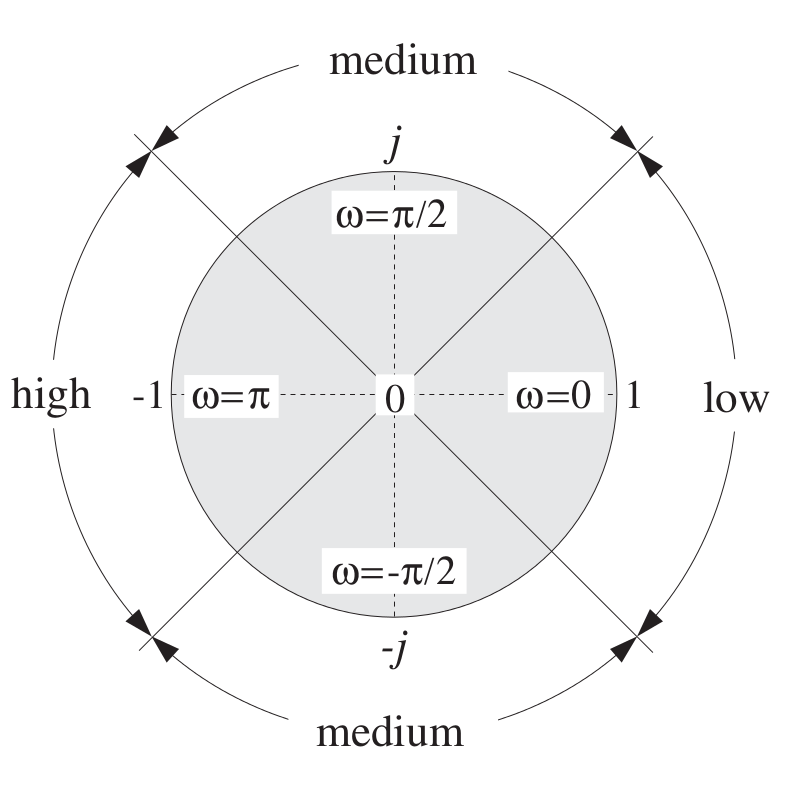
\includegraphics[width=6cm]{./picture/freq_spect}
\end{multicols}

Another useful relationship is Parseval’s equation, which relates the total energy of a sequence to its spectrum: 
\begin{align}
\sum_{n=-\infty}^{\infty} |x(n)|^2= \frac{1}{2\pi} \int\limits_{-\pi}^{\pi} |X(\omega)|^2 d\omega && \text{(Parseval)} \notag
\end{align}

Some DTFT-Transforms: \\ \\
\begin{tabularx}{0.7\textwidth}{|l|X|}
	\hline
	$\delta[n]$ &	$X_{2\pi}(\omega) = 1$ \\
	\hline 	
	$\delta[n-M]$ &	$X_{2\pi}(\omega) = e^{-i\omega M}$ \\
	\hline
	$u[n]$ & %$X_{2\pi}(\omega) = \frac{1}{1-e^{-i \omega}} + \pi \sum_{k=-\infty}^{\infty} \delta (\omega - 2\pi k) $ \\ & 	
	$X(\omega) = \frac{1}{1-e^{-i \omega}} + \pi \cdot \delta (\omega) $ \\
	\hline
	$e^{-i \omega_0 n}$ &	$X(\omega) = 2\pi\cdot \delta (\omega +\omega_0),     -\pi \leq \omega_0 < \pi$ \\
	\hline
	$\cos(\omega_0 n) $ & $X(\omega) = \pi [\delta (\omega +\omega_0)+\delta (\omega -\omega_0)],     -\pi < \omega_0 < \pi $\\
%	\\ & $X_{2\pi}(\omega) = \pi \sum_{k=-\infty}^{\infty} \left[ \delta (\omega - \omega_0 - 2\pi k) + 
%	\delta (\omega + \omega_0 + 2\pi k) \right] $ \\
	\hline
	$\sin(\omega_0 n) $ & $X(\omega) = -j \pi \delta(\omega - \omega_0) + j \pi \delta(\omega + \omega_0)$\\
%		$X_{2\pi}(\omega) = \frac{\pi}{i} \sum_{k=-\infty}^{\infty} \left[ \delta (\omega - \omega_0 - 2\pi k) 
%	- \delta ( \omega + \omega_0 + 2\pi k) \right] $  	\\
	\hline
\end{tabularx} \\ \\

Some Z-Transforms:\\
\begin{tabularx}{0.6\textwidth}{|X|X|X|}
	\hline
	\textbf{x(n} ) & \textbf{X(z}) & \textbf{ROC} \\
	\hline
	$u(n)$ & $\frac{1}{1 - z^{-1}}$ & $|z|>1$ \\
	\hline
	$-u(-n-1)$ & $\frac{1}{1 - z^{-1}}$ & $|z|<1$ \\
	\hline
	$(-1)^n u(n)$ & $\frac{1}{1 + z^{-1}}$ & $|z|>1$ \\
	\hline
	$-(-1)^n u(-n-1)$ & $\frac{1}{1 + z^{-1}}$ & $|z|<1$ \\
	\hline
	$a^n u(n)$ & $\frac{1}{1 - az^{-1}}$ & $|z|>|a| \quad$ (causal) \\
	\hline
	$-a^n u(-n-1)$ & $\frac{1}{1 - az^{-1}}$ & $|z|<|a| \quad$ (acausal) \\
	\hline
	$e^{\alpha n}$ & $\frac{z}{z-e^{\alpha}}$ & \\
	\hline
	$\cos(\omega n)$ & $\frac{z(z-\cos(\omega))}{z^2 -2z\cos(\omega) + 1}$ & \\
	\hline
	$\sin(\omega n)$ & $\frac{z\sin(\omega)}{z^2 -2z\cos(\omega) + 1}$ & \\
	\hline
	$A\delta(n)$ & $A$ & \\
	\hline
\end{tabularx}
\begin{minipage}[b][5.4cm][t]{5cm}
	For real valued discrete time sequences:\\
	$X(\omega)^* = X(-\omega)$ \\
	$|X(\omega)| = |X(\omega)|$\\
	$argX(\omega) = -argX(-\omega)$
\end{minipage}


\subsection{Inverse z-Transforms\buchSeite{202-204}}

$X(z) = \dfrac{N(z)}{D(z)} = \dfrac{N(z)}{(1-p_1z^{-1})(1-p_2z^{-1})\ldots(1-p_Mz^{-1})} = 
A_0 + \dfrac{A_1}{1-p_1z^{-1}} + \ldots + \dfrac{A_M}{1-p_Mz^{-1}}$

with $A_0 = X(z)|_{z=0}$ \\

\textbf{PBZ\buchSeite{203}:} for Order of $N(z) <$ Order of $D(z)$ \\
\[A_i = [(1-p_iz^{-1})X(z)]_{z=p_i} = \left[\frac{N(z)}{\prod\limits_{j\neq i}(1-p_jz^{-1})}\right]_{z=p_i}\]

\textbf{Euler:}

\begin{align}
\cos(\alpha) = \frac{e^{j\alpha} + e^{-j\alpha}}{2}
&& \sin(\alpha) = \frac{e^{j\alpha} - e^{-j\alpha}}{2j} && 
    {e}^{\pm jn\omega} = \cos{n\omega} \pm j \sin{n\omega} \notag\\
e^{j\frac{\pi}{2}n} = j^n & & e^{-j\frac{\pi}{2}n} = (-j)^n &&
e^{jn\pi}=e^{-jn\pi}=(-1)^n \notag
\end{align}
$(1-ae^{j\omega}z^{-1})(1-ae^{-j\omega}z^{-1}) = 1 - 2a\cos(\omega)z^{-1}+a^2z^{-2}$


